\documentclass[a0, portrait]{a0poster}
\usepackage[ngerman, welsh, english]{babel} % welsh seems to be needed for blindtext
\usepackage[amssymb]{SIunits}
\usepackage{amsmath, amssymb}
\usepackage{multicol, fancybox}
\usepackage{color,graphicx}
\usepackage{wallpaper}
\usepackage{pdfposter}
\usepackage{blindtext}
\usepackage[utf8]{inputenc}
\usepackage{calc}
\usepackage{booktabs} % beautiful tabs
\usepackage{layouts}

%-----------------------------------------------------------------------
% some settings for your poster:
\newcommand{\postertitle}{A fancy poster on some advanced topic} % title of the poster
\newcommand{\posterauthors}{Alexander Ebersp\"acher} % authors
\newcommand{\authorsinst}{Otto-von-Guericke-Universit\"at, Magdeburg} % author's affiliations, institutes
\newcommand{\conference}{{A nice Conference, 2042\\Beautyville\\Germany}} % conference name and date
\graphicspath{{images/}} % subfolder for the figures/images
\newcommand{\instlogo}{NAT_SIGN_druck2} % filename of the logo
\newcommand{\columnnumber}{3} % number of columns on the poster
\definecolor{topcolor}{RGB}{255,255,255} % color of page top (used for color gradient)
\definecolor{bottomcolor}{RGB}{51, 181, 64} % color of page bottom (used for color gradient)
\newcommand{\topcolorpercentage}{100} % top color opacity: 100 full color, 0: fully transparent
\newcommand{\bottomcolorpercentage}{11} % bottom color opacity: 100 full color, 0: fully transparent

%-----------------------------------------------------------------------
% usually, you don't want to change anything below here.
% the contents of your poster goes to content.tex, which will be loaded
% below.

\hypersetup{colorlinks,
  breaklinks=true,
  linkcolor=black,
  urlcolor=black,
  citecolor=black,
  bookmarksnumbered,
  pdfauthor={\posterauthors},
  pdftitle={\postertitle}}


% if the column spacing is bad, maybe change something here:
\setlength{\columnsep}{7.5ex} % separation of the columns

\begin{document}

\begin{minipage}{0.98\textwidth}
  \begin{center}

    %-----------------------------------------------------------------------
    % color gradient for the page
    \begin{tikzpicture}[remember picture, overlay]
      \node[inner sep=0pt, rectangle, top color=topcolor!\topcolorpercentage, bottom color=bottomcolor!\bottomcolorpercentage, minimum width=\paperwidth, minimum height=\paperheight] at (current page.center) {};
    \end{tikzpicture}
    %-----------------------------------------------------------------------

    %-----------------------------------------------------------------------
    % insert the header box
    \titlebox{\postertitle}{\posterauthors}{\authorsinst}{\instlogo}{\conference}
    %-----------------------------------------------------------------------

    % add star here (multicols*) and in \end{multicols} for unbalanced columns:
    \begin{multicols}{\columnnumber}[]

      %-----------------------------------------------------------------------
      % load content.tex
      % all the content of the poster goes here.
% uses greenboxes, blueboxes, redboxes as shown below.

\begin{greenbox}{Some info on lengths}
\begin{center}
\begin{tabular}[]{l c}
\toprule
\multicolumn{2}{c}{Lengths, width and margins}\\
\midrule
hoffset & \the\hoffset\\
voffset & \the\voffset\\
parskip & \the\parskip\\
parindent & \the\parindent\\
leftmargin &  \the\leftmargin\\
rightmargin & \the\rightmargin\\
topmargin & \the\topmargin\\
oddsidemargin & \the\oddsidemargin\\
evensidemargin & \the\evensidemargin\\
textwidth & \the\textwidth\\
textheight & \the\textheight\\
paperwidth & \the\paperwidth\\
paperheight & \the\paperheight\\
headheight & \the\headheight\\
footskip & \the\footskip\\
%footheight= \the\footheight\\
\bottomrule
\end{tabular}
\end{center}
\end{greenbox}

%-----------------------------------------------------------------------
\begin{greenbox}{Abstract}
\blindtext
\end{greenbox}
%-----------------------------------------------------------------------


%-----------------------------------------------------------------------
\begin{greenbox}{A first box}
In the first box, there shall be some
\[ \mathrm{F}_{\mathrm{or}}^{\mathrm{mul}} = as \]
and furthermore,
\begin{align*}
some &= fancy\\
1 &\equiv 1
\end{align*}
environment shall be used.
\end{greenbox}
%-----------------------------------------------------------------------

%-----------------------------------------------------------------------
\begin{greenbox}{The second box}
\begin{itemize}
	\item First
	\item Second
	\item Third and forth
\end{itemize}
\end{greenbox}
%-----------------------------------------------------------------------

%-----------------------------------------------------------------------
\begin{greenbox}{Graphics work, too!}
Some beautiful plot is this one:\\ % short lines benefit from manual line breaks
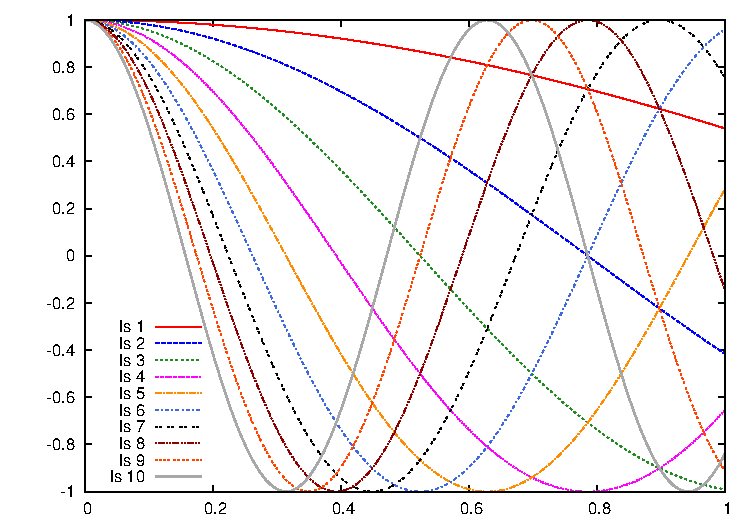
\includegraphics[width=0.9\textwidth]{images/colortest}\\
It shows many Gnuplot linestyles with plenty of
\begin{enumerate}
	\item thickness
	\item contrast
	\item beauty
\end{enumerate}

\end{greenbox}
%-----------------------------------------------------------------------

\columnbreak

%-----------------------------------------------------------------------
\begin{greenbox}{Some formulas}
A nice formula is\\
\begin{align*}
-1 = \mathrm{e}^{-\mathrm{i}\pi}\, .
\end{align*}
\end{greenbox}
%-----------------------------------------------------------------------

%-----------------------------------------------------------------------
\begin{greenbox}{Blocks}

Blocks do work, too:\\
\begin{greenblock}{Block title}{0.95\textwidth} % hier ein grüner block
Block content. Block formula:\\
\[ a^2+b^2=c^2\]
\end{greenblock}

Also, there is text below blocks.

\begin{minipage}{\textwidth}
	
\begin{minipage}{0.475\textwidth}
\begin{blueblock}{Blocks next to each other}{0.9\textwidth}
In blue, this time.
\end{blueblock}
\end{minipage}
\begin{minipage}{0.475\textwidth}
\begin{redblock}{Important block}{0.9\textwidth}
Muy importante!
\end{redblock}
\end{minipage}
\end{minipage}

\end{greenbox}

\begin{redbox}{Outlook}
Outlook is either something you want to do next or a M\$ program.
\end{redbox}

\begin{bluebox}{Blue velvet}
Boxes in other colors work as well.\\
Even blue ones.
\end{bluebox}

%-----------------------------------------------------------------------


    \end{multicols}

  \end{center}
\end{minipage}

\end{document}
